\documentclass[12pt,A4,onecolumn,french]{article}
\usepackage[utf8x]{inputenc}
\usepackage{graphicx}

%%%%%%%%%%%%%%%%%%%%%%%%%%%%%% User specified LaTeX commands.

\usepackage[top=0.6in, bottom=0.5in, left=0.75in, right=0.75in]{geometry}


%\usepackage{mathrsfs}

\usepackage{listings}


\usepackage{babel}



\begin{document}
%\usepackage{epsfig}
\thispagestyle{empty} %\usepackage[utf8x]{inputenc}



\date{}


\title{ UE MEMS \\ TP 2 \\ Dimensionnement d'un capteur d'accéleration et de son circuit de mesure}


\author{\hspace{1cm}Dimitri Galayko}

\pagestyle{empty}


\maketitle

\bibliographystyle{ieeetr}



\section{Introduction}
Ce TP représente la première partie du travail de conception d'un système complet permettant de mesurer l'accélération. Ce système est composé des parties suivantes : 

-- Un capteur mécanique composé de résonateur et de transducteurs électrostatiques associés, 

-- Un circuit d'interface permettant de mesurer la valeur de la capacité du transducteur qui représente le déplacement instantané de la masse mobile, 

-- Un circuit de conversion / asservissement permettant de numériser le signal et d'améliorer les performances intrinsèques du capteur électromécanique.  

Dans cette partie, nous allons concevoir et tester les deux premiers blocs de cette architecture. 

La géométrie du dispositif mécanique est inspirée de l'article [1]. Cet article vous est distribué, vous êtes invités à le lire. 

Ce TP utilise la modélisation spice des systèmes électromécaniques. La méthodologie de la modélisation a été présenté dans le TP1. 

\section{Dimensionnement du capteur}

\subsection{Dimensionnement du résonateur}
Le résonateur est composé d'une masse mobile et des ressorts de suspension. 

D'après la table 1 de l'article [1], la masse mobile peut être vue comme une
"brique" 120 $\mu$m de hauteur, et 3 mm $\times$ 5 mm de surface. Etant donné la
densité volumique du silicium de 2300 $kg\cdot m^{-3}$, nous obtenons pour la masse la valeur de $m=4.14e-6$ kg.

La masse joue un très grand rôle dans la mesure de l'accélération, dans la mesure où l'accélération ne se manifeste qu'à travers la force inertielle qui est proportionnelle à la masse ($m\cdot a_{ext}$). Pour cette raison, la masse d'accéléromètre est toujours relativement grande.   

La géométrie de la partie mobile est dimensionnée de sorte à avoir un résonateur à facteur de qualité de 0.3. Un facteur de qualité aussi faible permet d'avoir un système de type "filtre passe-bas". La fréquence de coupure ciblé est de 500 Hz 

\emph{\bf A faire: } Calculez la valeur de la raideur du ressort ($k$) permettant d'obtenir cette fréquence de coupure et ce facteur de qualité.    


Une fois la constante de raideur calculée, on peut dimensionner les ressort. On se base sur la fig. 2 de l'article [1]. On voit que le ressort est réalisé à partir de 4 poutres fonctionnant en mode "guidée" (cf. la table présentée en cours 2). 

\emph{\bf A faire: }Sachant que la hauteur des ressorts est fixé à 120 $\mu$m, trouvez le rapport de forme des deux autres dimensions du ressort.

\subsection{Dimensionnement des capacités variables}

D'après le dessin de la fig. 2, il y a deux paires identiques de capacités variables (une en haut et une en bas du dessin). Une vue élargie d'une de ses paires est donné fig. \ref{fig:geometrie}. On voit, que lorsque la masse mobile se déplace vers la droite (dans le sens conventionnel positif), la capacité de gauche ($C_{plus}$) augmente, la capacité de droite ($C_{moins}$) diminue. Cette variation différentielle peut être mesurée par des circuits électroniques appropriés.

\begin{figure}
 \centering
 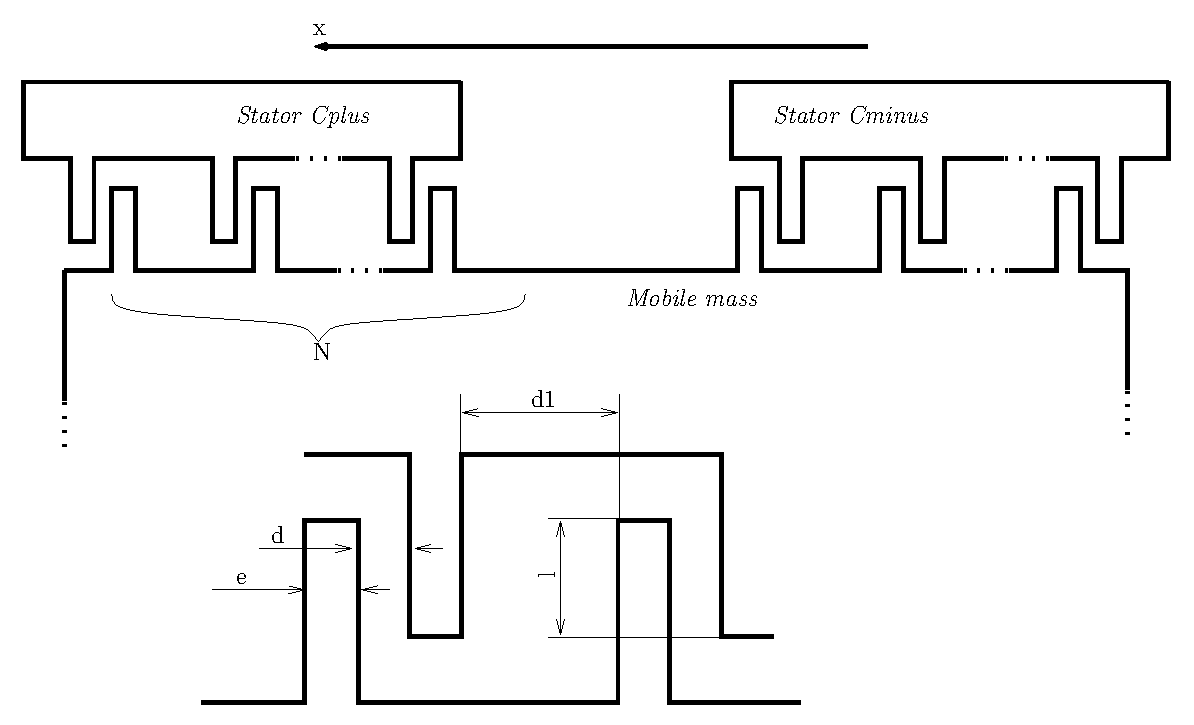
\includegraphics{capa_geometry.eps}
 \caption{Géométrie des capacités variables \label{fig:geometrie}}
\end{figure}

Les dimensions des capacités sont données fig. \ref{fig:geometrie}. Nous vous proposons les valeurs suivantes : 

d=4 $\mu$m, d1=10 $\mu$m, l=100 $\mu$m, e=4 $\mu$m, N=300. 

Ici $N$ est le nombre de capacités de chaque transducteur. 

La structure étant symétrique par rapport à l'axe central horizontal, chaque transducteur possède sa réplique, avec laquelle il est connectée en parallèle. Il faudra donc penser à introduire un facteur 2 dans le calcul de la capacité.  

\emph{\bf A faire :} Calculez la valeur des deux capacités variables au repos. Donnez les valeurs des capacités pour déplacement 1, 2 et 3 $\mu$m. 

\emph{\bf A faire :} En supposant que le déplacement maximal de la masse mobile est de 3 $\mu$m (3/4 du gap), donnez la valeur maximale de l'accélération qu'un tel système est capable de mesurer.

\subsection{Test de comportement mécanique}

Dans cette partie, on étudiera le comportement mécanique de du dispositif MEMS de l'accéléromètre. Le nouveau dispositif, dont le modèle est présenté fig. \ref{fig:modele_transducteur}, contient un résonateur du second ordre et un transducteur différentiel à mouvement vertical. Ainsi, dans le nouveau système, il y a deux transducteurs. Le modèle spice du transducteur (un sous-circuit MEMS\_accelerometer) possède les terminaux suivants: 

-- Un terminal mécanique d'entrée \emph{f\_ext} auquel on applique une tension qui représente la force $F$ agissant sur la masse. Il s'agit d'une force externe. Pour l'application de l'accéléromètre, il faudra la définir comme $F=-m\cdot a_{ext}$, où $a_{ext}$ est l'accélération externe à mesurer. Nous avons donc $F=V(f\_ext)$. 

-- "cplus", "common", "cminus": les électrodes électriques correspondant aux trois électrodes de la capacité variable différentielle formée par les transducteurs

-- les terminaux "pos", "capa\_plus", "capa\_minus" sont des terminaux dont les tensions donnent respectivement la position de la masse mobile, la capacité gauche et la capacité droite du transducteur. Ces terminaux sont définis uniquement pour pouvoir tester le système.  

Les paramètres du modèle sont les paramètres du transducteur (masse, raideur, amortissement), les paramètres des transducteur (le gap et l'aire de recouvrement) et la position des stoppeurs. Les valeurs par défaut du dispositif définies dans le fichier MEMS\_accelerometer.cir correspondent aux données de notre problème. Il ne faut pas les modifier.    

Le modèle du dispositif, appelé \emph{MEMS\_accelerometer}, vous est fourni, avec des commentaires détaillés.  

\begin{figure}
 \centering
 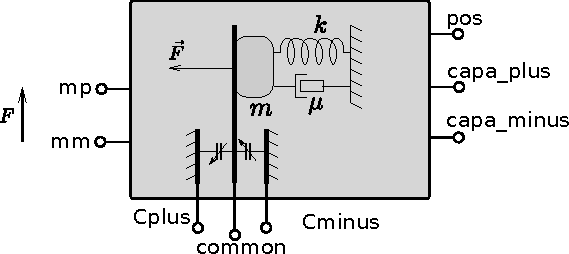
\includegraphics{accelerometer_model.pdf}
 \caption{ \label{fig:modele_transducteur}}
\end{figure}


\emph{\bf A faire :} En complétant le fichier de netlist test\_mechanique.cir, modélisez le résonateur soumis à une accélération externe constante de 1$g$. Les terminaux électriques sont connectés à la masse (on ne s'intéresse qu'à la partie mécanique). Observer le processus transitoire. Quelle est la position asymptotique de la masse mobile? Quelle sont les valeurs correspondantes des capacités ?
\emph{\bf A faire :} Calculez la transmission "intrinsèque" de l'accéléromètre, défini comme: 
\begin{eqnarray} 
\gamma=\frac{ C_{plus}-C_{minus}}{A_{ext}}
\end{eqnarray}

Le rôle de l'électronique sera de mesurer cette différence de capacités. 

\section{Mesure de la capacité}

Dans cette partie, on va mettre en oeuvre un circuit de mesure de la capacité différentielle. On testera deux architectures: l'une utilisant la technique de détection synchrone et l'autre utilisant la technique des capacités commutées. 

\subsection{Mesure par technique de capacité commuté}

\begin{figure}
 \centering
 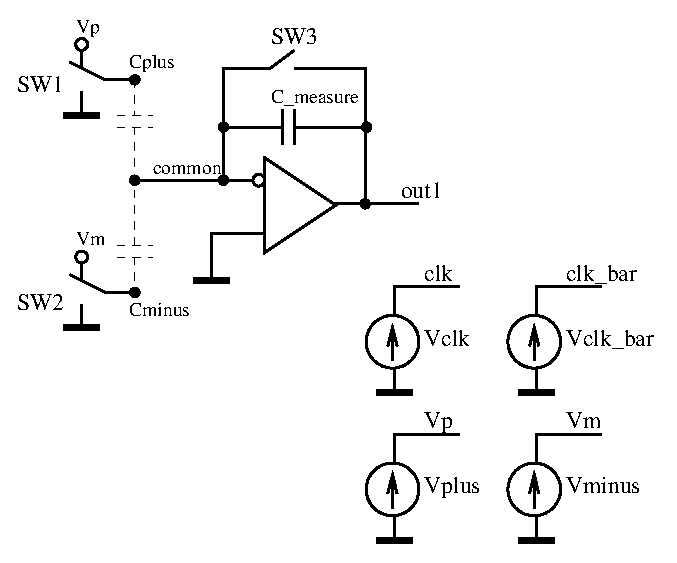
\includegraphics[width=0.6\textwidth]{measurement_capacom.eps}
 \caption{Circuit permettant d'effectuer une mesure d'une capacité différentielle par la technique des capacités commutées. Les positions des switches présenté sur le schéma correspondent à la phase 1 (état haut) de l'horloge clk. L'horloge clk\_bar est le complément numérique de l'horloge clk. L'état haut de clk\_bar met les switches dans les positions opposées à celles données sur le schéma. \label{fig:capacom}}
\end{figure}

Maintenant on étudie le circuit donné fig. \ref{fig:capacom}. 

Les switches commutent à fréquence 50 kHz, la valeur des tensions vp et
vm sont continue et valent +1 et - et -1 V. 

Le nouveau système est modélisé dans le fichier accelerometer\_capacom.cir. Les switches commandés sont réalisé par des modèles macroscopiques de ngspice. Pour les détails (interfaces, paramètre...), vous êtes invités à consulter le manuel de ngspice qui se trouve dans le répertoire d'installation du logiciel. 

Vous donnerez une valeur de 10 p à la capacité C\_measure. 

\emph{\bf A faire} : Calculez la formule donnant le rapport entre l'accélération et la tension de sortie.  Validez par modélisation avec $a_{ext}=1...4 g$. 

\emph{\bf A faire} : Quelle accélération provoque un déplacement de 3 $\mu$m ? Appliquez cette accélération et observez le phénomène de pull-in.  

\emph{\bf A faire:} Comment faut-il modifier le circuit (les paramètres) pour éviter le pull-in et ainsi pour mesurer des accélérations provoquant un déplacement jusqu'à 3 $\mu$m. 

\emph{\bf A faire:} Ajouter au circuit un dispositif échantillonneur-bloqueur
échantillonné d'une manière appropriée (pour cela vous devrez générer une horloge à part).

\emph{\bf A faire:} Appliquez une accélération sinusoidale d'amplitude 0.2g et de fréquences 100, 300, 400, 600, 900 Hz. Dessinez la fonction "transmission $\gamma$ - fréquence" et concluez sur le fonctionnement de l'accélérateur à hautes fréquences.  

\section{Bibliographie}
[1] B. V. Amini, R. Abdoulvand, F. Ayazi, A 4.5-mW closed-loop $\Sigma\Delta$ micro-gravity CMOS SOI accelerometer, IEEE journal of solid state circuits, vol. 41, no. 12, december 2006
\end{document}
